\section{Diskussion}

Das kleinere, ausschließlich mit literaturbasierten Features trainierte Modell erreichte mit 87\% bereits eine hohe Präzision.
Dies kann dahingehend interpretiert werden, dass die genutzten Features grundsätzlich geeignet sind um verschwörungstheoretische Texte von (wissenschafts-) journalistischen zu Unterscheiden.

Die verwendete \textit{LightGBM} Software erlaubt es die Bedeutung einzelner Features für das erstellte Modell abzuschätzen.
Das Feature mit dem höchsten Informationszuwachs (Gain) für das Modell ist die Anzahl der internen Links (Gain = $0.12$).
Die Anzahl der externen Links hingegen bot einen deutlich geringeren Gain ($0.076$) für das Modell.
Dies ist insofern bemerkenswert, als dass die in der Literatur gemachten Beobachtungen wie etwa die von \textcite[10]{soukup_2008} hätten vermuten lassen, dass die Verknüpfung mit externen Quellen ein wichtigeres Merkmal ist als die mit internen.

Die nächstwichtigsten Features sind die Anzahl der eingebundenen Bilder (Gain = $0.1$), die Summe der Sentimente ($0.1$) und der Anteil an zitierten Text ($0.9$).
Interessant ist hier noch, dass, anders als die Summe an Sentiment Scores, der Betrag der Sentiment Scores für die Klassifizierung relativ unbedeutend ist (Gain = $0.018$).
Dies kann zum einen daran liegen, dass diese Werte nicht vollständig unabhängig voneinander sind und der Trainingsalgorithmus deshalb u.U. nur einen der Werte berücksichtigt.\footnote{Baum-basierte Verfahren sind meist in der Lage relevante Features zu einem gewissen Grad selbst zu selektieren.}
Zum anderen kann es aber auch ein Indiz dafür sein, dass Verschwörungstheoretische Texte nicht notwendigerweise allgemein emotionaler sind, aber im Schnitt deutlich negativere Sentimente Transportieren.
Dies bestätigt sich auch an den Durchschnittswerten der Sentimentsumme ($\overline{X}_1 = -4.22$ gegenüber $\overline{X}_0 = -1.35$).

Die meisten anderen Features lieferten dem Modell einen mittelgroßen Informationszuwachs, besonders wenig nützlich waren vor allem Features, die mehr oder weniger mit anderen Features zusammenhängen (die Summe positiver bzw. negativer Sentimente, Zahl der direkten Zitate, etc.), was durchaus erwartbar ist.
Ebenso relativ wenig hilfreich waren die Menge an Negationen, an Zahlenangaben sowie allgemein an eingebetteten Medien (Twitter, Youtube, Sonstige).
Eine Erklärung für letztere könnte dabei aber auch schlicht sein, dass herkömmliche Medien inzwischen solche Medien auch häufiger einbinden und in diesem stilistischen Merkmal sich den Verschwörungstheorien angenähert haben.

Es bleibt anzumerken, dass Verfahren des maschinellen Lernens, wie hier Gradienten-Boosting, komplexe Systeme sind und die Interpretation solcher Ergebnisse immer mit Vorsicht vorgenommen werden sollte.

\begin{figure}[h]
    \centering
    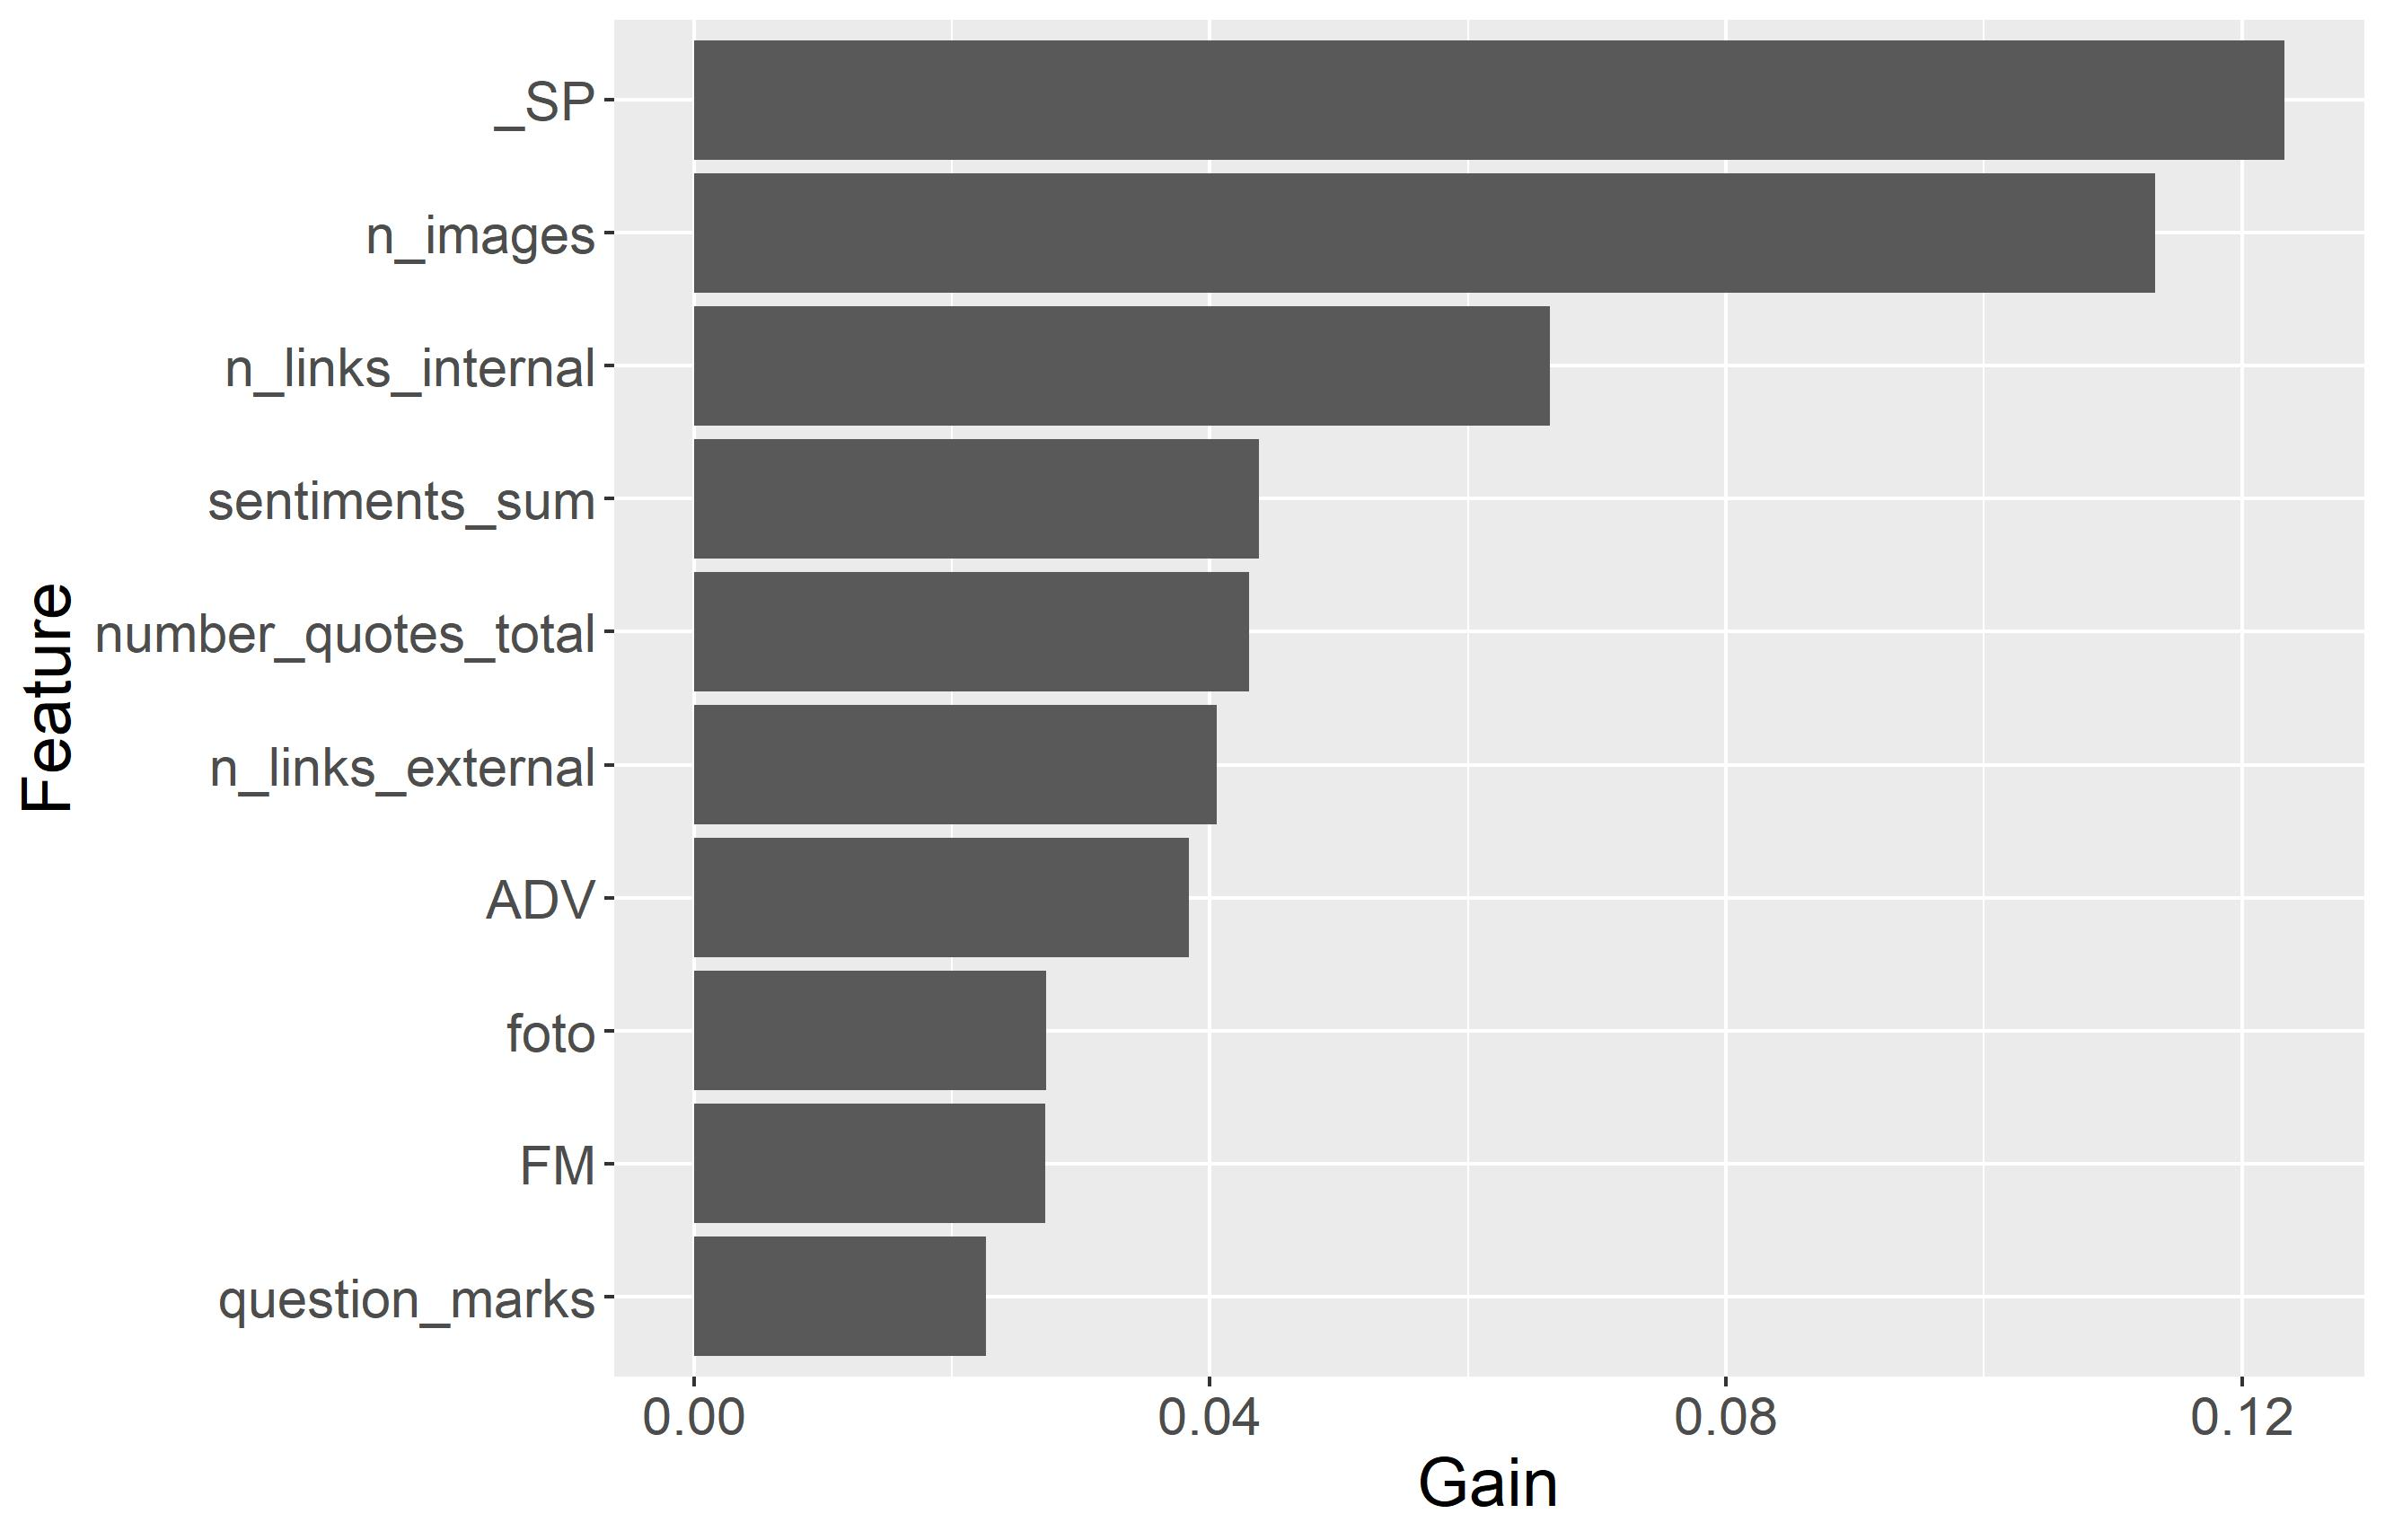
\includegraphics[scale=0.45]{graphics/top_10_features.jpg}
    \caption{Top-10 Features nach Bedeutung für das Modell. (Namen in Großbuchstaben = Part-of-Speech Tag; Namen in Kleinbuchstaben = tf-idf Worthäufigkeit; Benannte Features = Auf Literatur basierende Statistiken)}
    \label{top-features}
\end{figure}

\FloatBarrier

Das vollständige Modell erreichte mit fast 98\% eine sehr gute Präzision, auch Spezifität und Sensitivität sind auf ähnlich hohem Niveau.
Es kann zuverlässig zwischen den Verschwörungstheoretischen Texten und dem Vergleichskorpus unterscheiden.
Eine Betrachtung der wichtigsten Features aus Grafik \ref{top-features} zeigt zunächst, dass viele der auch für das kleinere Model wichtigen Features wieder von großer Bedeutung sind (Zahl der Bilder, Zahl der internen Links, Summe der Sentiment Scores und Anteil von zitiertem Text).
Einige der Wortfrequenzen mit dem meisten Einfluss auf die Klassifizierungen sind Foto, Krieg, Merkel und Regierung.
Die meisten davon sind wenig überraschende Ergebnisse, die Verwendung von Worten aus Themenbereichen wie Krieg und Macht ist in der Literatur gut belegt, etwa bei \textcite[150]{stumpf_2019} oder \textcite[25]{uscinski_2014}.
Unter den wichtigen POS Tags sind Leerzeichen, Adverben, fremdsprachiger Text und Coordinating Conjunctions (also Wörtern wie und, oder, aber, etc. \parencite[vgl.][]{smith_2003}).
Interessant ist auch, dass die Zahl der Fragezeichen im kleineren Modell zwar kaum relevant ist, im größeren Modell aber unter den 10 einflussreichsten Features.

Eine mögliche Erklärung für die überraschend gute Leistung des trainierten Modells ist, dass die relativ geringe Vielfalt, insbesondere im Untersuchungskorpus, einen Teil zu der guten Leistung beigetragen hat.
Auch wenn etwa für \textit{Watergate.tv} mehrere Autor:innen schreiben, ist zu vermuten dass die totale Anzahl an Autor:innen im Korpus im niedrigen zweistelligen Bereich liegt.
Da in der Modellerstellung mit den Part-of-Speech Tags auch eher stilistische Features genutzt werden, ist es durchaus möglich, dass ein Teil der Leistung des Modells weniger auf verschwörungstheoretischen Merkmalen beruht als auf dem Stil der individuellen Autor:innen.

Dies könnte ein Faktor sein, der es unwahrscheinlicher macht, dass das vorgestellte Modell gut generalisiert.